\documentclass[letterpaper]{article} % DO NOT CHANGE THIS
\usepackage{aaai2027}  % DO NOT CHANGE THIS
\usepackage[hyphens]{url}  % DO NOT CHANGE THIS
\usepackage{graphicx} % DO NOT CHANGE THIS
\urlstyle{rm} % DO NOT CHANGE THIS
\def\UrlFont{\rm}  % DO NOT CHANGE THIS
\usepackage{natbib}  % DO NOT CHANGE THIS AND DO NOT ADD ANY OPTIONS TO IT
\usepackage{caption} % DO NOT CHANGE THIS AND DO NOT ADD ANY OPTIONS TO IT
\frenchspacing  % DO NOT CHANGE THIS

% Recommended for better-looking tables
\usepackage{booktabs}

\pdfinfo{
/TemplateVersion (2027.1)
}

\setcounter{secnumdepth}{0}

% ------------------------------------------------------------------
% NOTE TO AUTHOR (delete before submission):
% 1. Replace the affiliation placeholder below with your institution.
% 2. The two tables marked "REAL-DATA RESULTS" contain the completed
%    controlled-simulation numbers. After `make real-all` finishes,
%    add the LoCoMo and LongMemEval tables where indicated by the
%    commented TODO blocks.
% ------------------------------------------------------------------

\title{When Should Agents Forget? A Controlled Comparison of Forgetting Policies in Bitemporal Agent Memory}
\author{
    Hao Wang\textsuperscript{\rm 1},
    Nandan Hemanth\textsuperscript{\rm 1}\corresponding
}
\affiliations{
    \textsuperscript{\rm 1}Department of Applied Artificial Intelligence, Your University\\ % TODO: replace with real affiliation
    theuniverseisflat101@gmail.com
}

\begin{document}

\maketitle

\begin{abstract}
Long-lived language model agents accumulate memories that go stale. A fact that was true when it was stored, such as where a user lives, is later contradicted by an update, yet retrieval keeps surfacing the old value. We study a simple question: when should an agent forget? We present DRIFT, an experimental framework in which the forgetting policy is the only independent variable. The memory substrate, fact extraction, retrieval, and judging are held fixed, so measured differences between policies are attributable to the policies themselves. On a bitemporal knowledge graph, where every fact carries a validity interval and an ingestion time, we compare six policies: a no-memory floor, an append-only baseline, time-to-live decay, contradiction-driven invalidation, novelty-gated writes, and periodic consolidation by a language model. We measure accuracy together with a separate staleness rate, the fraction of answers that contain a superseded fact. In controlled experiments, contradiction-driven invalidation removes staleness entirely while preserving recall of old but still valid facts, and this advantage is unchanged across three multi-agent topologies, including a shared memory written by five agents where every invalidation crosses writer boundaries. A time-blind structural ablation shows that graph structure alone is not sufficient: consolidating by structural support performs worse than not forgetting at all, because stale facts accumulate corroboration over time. Our results suggest that the representation, not a learned scoring function, does most of the work in memory hygiene.

Code and data: \url{https://github.com/NandanHemanth/DRIFT}
\end{abstract}

\section{Introduction}

Language model agents are increasingly deployed across sessions that span weeks or months. To act coherently they store facts about their users and their environment in an external memory, and the size of this memory grows without bound unless something is removed. The question of what to remove is usually answered by ad hoc heuristics: expire old entries, deduplicate similar ones, or ask a language model to tidy the store periodically. Recent work suggests these heuristics are not harmless. \citet{zhang2026faulty} show that memories continuously rewritten by a language model degrade below a no-memory baseline. \citet{patel2026supersede} measure a drop from 92\% to 77\% accuracy on knowledge-update questions when a frontier model must answer from self-maintained memory rather than full context. \citet{chao2026stale} find that even the best evaluated system resolves conflicting memories correctly only 55.2\% of the time.

These findings share a common failure mode that we call staleness: the agent answers with a fact that was true once and has since been superseded. Staleness is invisible to plain accuracy metrics on static recall benchmarks, because an agent can score well on most questions while confidently repeating outdated facts on the questions that matter. It is also the failure mode that forgetting is supposed to fix. Yet published evaluations compare complete memory systems against each other, where the storage format, the retrieval method, and the forgetting behavior all differ at once. From such comparisons one cannot conclude which component caused an observed difference.

We take a narrower approach. We fix a memory substrate, a bitemporal knowledge graph in the style of Zep and Graphiti \citep{rasmussen2025zep}, where each fact records both the interval during which it was valid in the world and the time at which the agent learned it. On top of this fixed substrate we vary only the forgetting policy, and we measure staleness separately from accuracy. The substrate matters for one specific reason: when a new fact contradicts an old one on a functional relation such as \texttt{lives\_in}, the graph closes the old fact's validity interval instead of deleting it. Whether a fact is superseded therefore becomes a property the policy can read, rather than a judgment the policy must make.

We ask four questions. First, how often does an append-only memory actually surface superseded facts? Second, which of the common policy families gives the best trade-off between accuracy, staleness, and cost? Third, does a policy that reads the graph's temporal structure beat policies that rely on age, similarity, or a language model's judgment? Fourth, do the answers change when memory is used the way agent systems actually use it, with several agents writing to a shared store, agents observing only part of the interaction history, or an orchestrator routing questions to specialist workers?

Our contributions are as follows.
\begin{itemize}
\item DRIFT, an open framework for controlled comparison of forgetting policies. The core has no third-party dependencies, every language model call is cached by content hash, and all experiments in this paper can be reproduced with single commands.
\item A staleness metric that is measurable by construction, because our evaluation data annotates each state-change question with the superseded answer.
\item A controlled comparison of six policies spanning the design space, including a no-memory floor and an append-only baseline, across single-agent and three multi-agent topologies with up to five heterogeneous writer agents.
\item A structure-versus-time ablation. A policy that consolidates using graph topology but ignores time performs worse than never forgetting, which localizes the benefit of structure-aware forgetting in the temporal fields specifically.
\end{itemize}

\section{Related Work}

\paragraph{Agent memory systems.} MemGPT introduced operating-system-style memory management for language models \citep{packer2023memgpt}. Mem0 \citep{chhikara2025mem0} targets production deployments, and A-MEM \citep{xu2025amem} organizes memories as evolving notes. Zep \citep{rasmussen2025zep} contributes the bitemporal temporal-knowledge-graph substrate that we adopt. These systems each implement some forgetting behavior, but it is entangled with the rest of the system, which is precisely the confound our design removes. A recent survey \citep{du2026memory} identifies learned forgetting and continual consolidation as open problems.

\paragraph{Forgetting and write control.} SAGE \citep{wang2026sage} gates memory writes by novelty, which corresponds to our policy P3. \citet{zhang2026faulty} document the risk of consolidation performed by a language model, which corresponds to our P4. Our contribution relative to both is the controlled setting: we run these mechanisms against alternatives on an identical substrate.

\paragraph{Staleness benchmarks.} STALE \citep{chao2026stale} and the knowledge-update analysis of \citet{patel2026supersede} both measure whether agents act on the current value of a changed fact. They evaluate existing systems; we complement them by explaining which policy choices produce the failures they observe.

\paragraph{Multi-agent shared memory.} GateMem \citep{ren2026gatemem} benchmarks governance in shared memories written by multiple principals and reports that no current method achieves utility, access control, and reliable forgetting at once. We do not address access control, but our shared-memory topology measures contradiction handling across writers under controlled policy variation, which their results motivate.

\paragraph{Evaluation data.} We build on LoCoMo \citep{maharana2024locomo} and LongMemEval \citep{wu2025longmemeval}, the standard long-term conversational memory benchmarks. LongMemEval's knowledge-update category is an independently constructed staleness probe.

\section{The DRIFT Framework}

\subsection{Memory substrate}

A fact is an edge $(s, p, o)$ with a surface text form and four lifecycle fields: $t_{\mathrm{valid}}$, the time the fact became true; $t_{\mathrm{invalid}}$, the time it stopped being true, if known; $t_{\mathrm{ingested}}$, the time the agent learned it; and an active flag that only a forgetting policy may clear. A set of functional predicates (\texttt{lives\_in}, \texttt{works\_at}, and similar) admit one true object per subject at a time. When a fact arrives whose subject and predicate match an existing active fact but whose object differs, the older fact's validity interval is closed at the new fact's event time. Nothing is deleted at this point. History remains intact until a policy prunes it. Each fact also records provenance, the identity of the agent that wrote it, which our multi-agent analysis uses.

\subsection{Pipeline}

Sessions of conversation are converted to facts by a language model extraction prompt, followed by a deterministic pattern-matching pass that normalizes functional predicates. The second pass exists so that contradiction detection does not silently depend on extraction luck. Retrieval scores each active fact by a fixed mixture of embedding similarity (weight 0.6), lexical overlap (0.3), and recency (0.1), and returns the top $k=8$. The answering model sees only the retrieved facts and the question. A judge model from a different vendor family grades each answer against gold, and we also report token-level F1 as a check that does not depend on any judge.

\subsection{Policies}

Policies interact with memory through three hooks: a write gate, a maintenance step after each session, and a filter at retrieval time. Table~\ref{tab:policies} lists the six policies we compare. NOMEM disables retrieval entirely and serves as a floor: it shows what the answering model knows without any memory. P0 stores everything and never forgets, which is the natural baseline for an agent without a forgetting policy.

\begin{table}[t]
\centering
\small
\begin{tabular}{@{}lll@{}}
\toprule
ID & Policy & Mechanism \\
\midrule
NOMEM & No memory & retrieval disabled (floor) \\
P0 & No forgetting & append-only (baseline) \\
P1 & TTL decay & prune facts older than 35 days \\
P2 & Contradiction & hide superseded facts at retrieval, \\
   & invalidation & prune after 7-day grace period \\
P3 & Novelty gate & reject near-duplicate writes \\
P4 & LLM consolidation & periodic keep or drop review \\
P5 & Topology & structural-support consolidation, \\
   & consolidation & time-blind (ablation) \\
\bottomrule
\end{tabular}
\caption{The compared policies. P2 is the only policy that reads the bitemporal fields. P5 is structure-aware but ignores time, which isolates the contribution of the temporal fields.}
\label{tab:policies}
\end{table}

P2 requires no learning and no model calls. It excludes facts whose validity interval is closed from retrieval results and prunes them after a grace period. P5, the ablation, clusters the entity co-occurrence graph by label propagation and, within groups of competing facts on the same subject and predicate, keeps the fact whose object is corroborated by the most other facts in memory. P5 deliberately never consults a timestamp.

\subsection{Multi-agent topologies}

Production agent systems rarely have a single writer. We therefore rerun every policy under three topologies while holding everything else fixed. In the \emph{shared} topology, $n$ agents take turns ingesting an interleaved timeline of sessions into one graph, so a contradiction is typically written by a different agent than the fact it supersedes. In the \emph{independent} topology, each agent has a private graph and observes a random 80\% of sessions, and we report the mean and standard deviation across agents. In the \emph{orchestrator} topology, a router model assigns each question to one of several specialist workers that share a single memory. Workers can be different model families. Our largest configuration uses five writer agents backed by five different model families.

\subsection{Reproducibility}

The framework core uses only the Python standard library. A deterministic offline provider and a hashing embedder allow the full pipeline to run without any network access, which we use for harness validation and unit tests (28 tests). Every real language model call is cached on disk under a content hash of provider, model, prompt, and temperature, so interrupted experiments resume without repeated calls and completed experiments can be re-derived exactly.

\section{Experimental Setup}

\paragraph{Data.} We use three datasets. A synthetic benchmark of two multi-session conversations over 58 simulated days contains planted fact updates (a move between cities, a job change), duplicated utterances as novelty probes, and 14 questions in three categories, where each state-change question is annotated with its superseded answer. This dataset is small by design: it is fully solvable by a deterministic answerer, so policy differences on it reflect the policies alone. LoCoMo \citep{maharana2024locomo} provides 10 very long multi-session conversations with about 1,986 questions; to fit free-tier judge quotas we evaluate a stratified sample of 300 questions proportional to the five question categories, keeping every conversation's full multi-week session history intact so long-horizon dynamics are unaffected and only the number of probe questions is reduced. LongMemEval \citep{wu2025longmemeval} provides a second, independently constructed benchmark whose knowledge-update category directly probes staleness.

\paragraph{Models.} The answer-model matrix covers five families: Llama-3.3-70B, gpt-oss-120B, Gemini 2.5 Flash, GLM-5.2, and MiniMax-M3. Extraction is fixed to one model, and the judge is fixed to Gemini 2.5 Flash, a different family from most answerers, with token-level F1 as a judge-free check. Embeddings for real runs use a locally served nomic-embed-text model.

\paragraph{Metrics.} We report accuracy by judge, token F1, staleness rate (the fraction of answers containing the annotated superseded fact), mean tokens per question, and the trajectory of active memory size. Multi-agent runs also report cross-writer invalidations and per-agent variance.

\section{Results}

We first report the controlled study, which uses the synthetic benchmark and the deterministic offline provider. These runs are exactly reproducible and isolate policy effects from model noise. We then describe the real-model experiments.

% ------------------------------------------------------------------
% REAL-DATA RESULTS (controlled study, completed)
% ------------------------------------------------------------------

\begin{table}[t]
\centering
\small
\begin{tabular}{@{}lcccc@{}}
\toprule
Policy & Acc. & F1 & Staleness & Facts \\
\midrule
P0 no forgetting & 0.714 & 0.243 & 0.286 & 12 \\
P1 TTL decay & 0.500 & 0.146 & 0.071 & 6 \\
P2 contradiction & \textbf{0.929} & \textbf{0.299} & \textbf{0.000} & 9 \\
P3 novelty gate & 0.714 & 0.243 & 0.286 & 11 \\
P4 LLM consolidation & 0.714 & 0.243 & 0.286 & 11 \\
P5 topology (ablation) & 0.500 & 0.192 & 0.071 & 5 \\
\bottomrule
\end{tabular}
\caption{Controlled study on the synthetic benchmark with the deterministic provider. Facts is the active memory size after all sessions. P2 dominates on all three quality metrics while pruning a quarter of memory relative to P0.}
\label{tab:controlled}
\end{table}

\paragraph{Staleness is systematic, not incidental.} In Table~\ref{tab:controlled}, the append-only baseline P0 answers every state-change question with the superseded fact. The reason is mechanical. The superseded statement is often lexically closer to the question than the update. ``I live in Boston, the city is great for museums'' shares more tokens with ``Which city does Alice live in?'' than ``I moved to Seattle recently'' does. Retrieval therefore prefers the stale fact, and better retrieval weights alone cannot fix a preference that comes from the data. This answers our first question: with no forgetting, 28.6\% of all answers, and 100\% of state-change answers, contain superseded facts.

\paragraph{Structure-blind forgetting trades one failure for another.} TTL decay (P1) reduces staleness fourfold but destroys recall of old facts that remain true, dropping overall accuracy below the baseline. Per-category results make the trade explicit: P1 answers 75\% of state-change questions correctly but 0\% of old-recall questions, while P0 does the opposite. The novelty gate (P3) and LLM consolidation (P4) shrink memory slightly but leave staleness untouched, because duplicates are not contradictions.

\paragraph{Reading the temporal structure wins.} P2 achieves the highest accuracy, zero staleness, and full recall of old facts, at no model-call cost. It forgets only what the graph proves is superseded, so it never pays the recall penalty that P1 pays.

\paragraph{Graph structure without time is worse than nothing.} The ablation P5 consolidates by structural support and reaches only 0.500 accuracy, below the append-only baseline. The mechanism is instructive: stale facts have been in memory longer, so more other facts corroborate them, and structural support therefore systematically votes to keep exactly the facts that should be removed. Structure awareness helps only when it is temporal structure.

\begin{figure}[t]
\centering
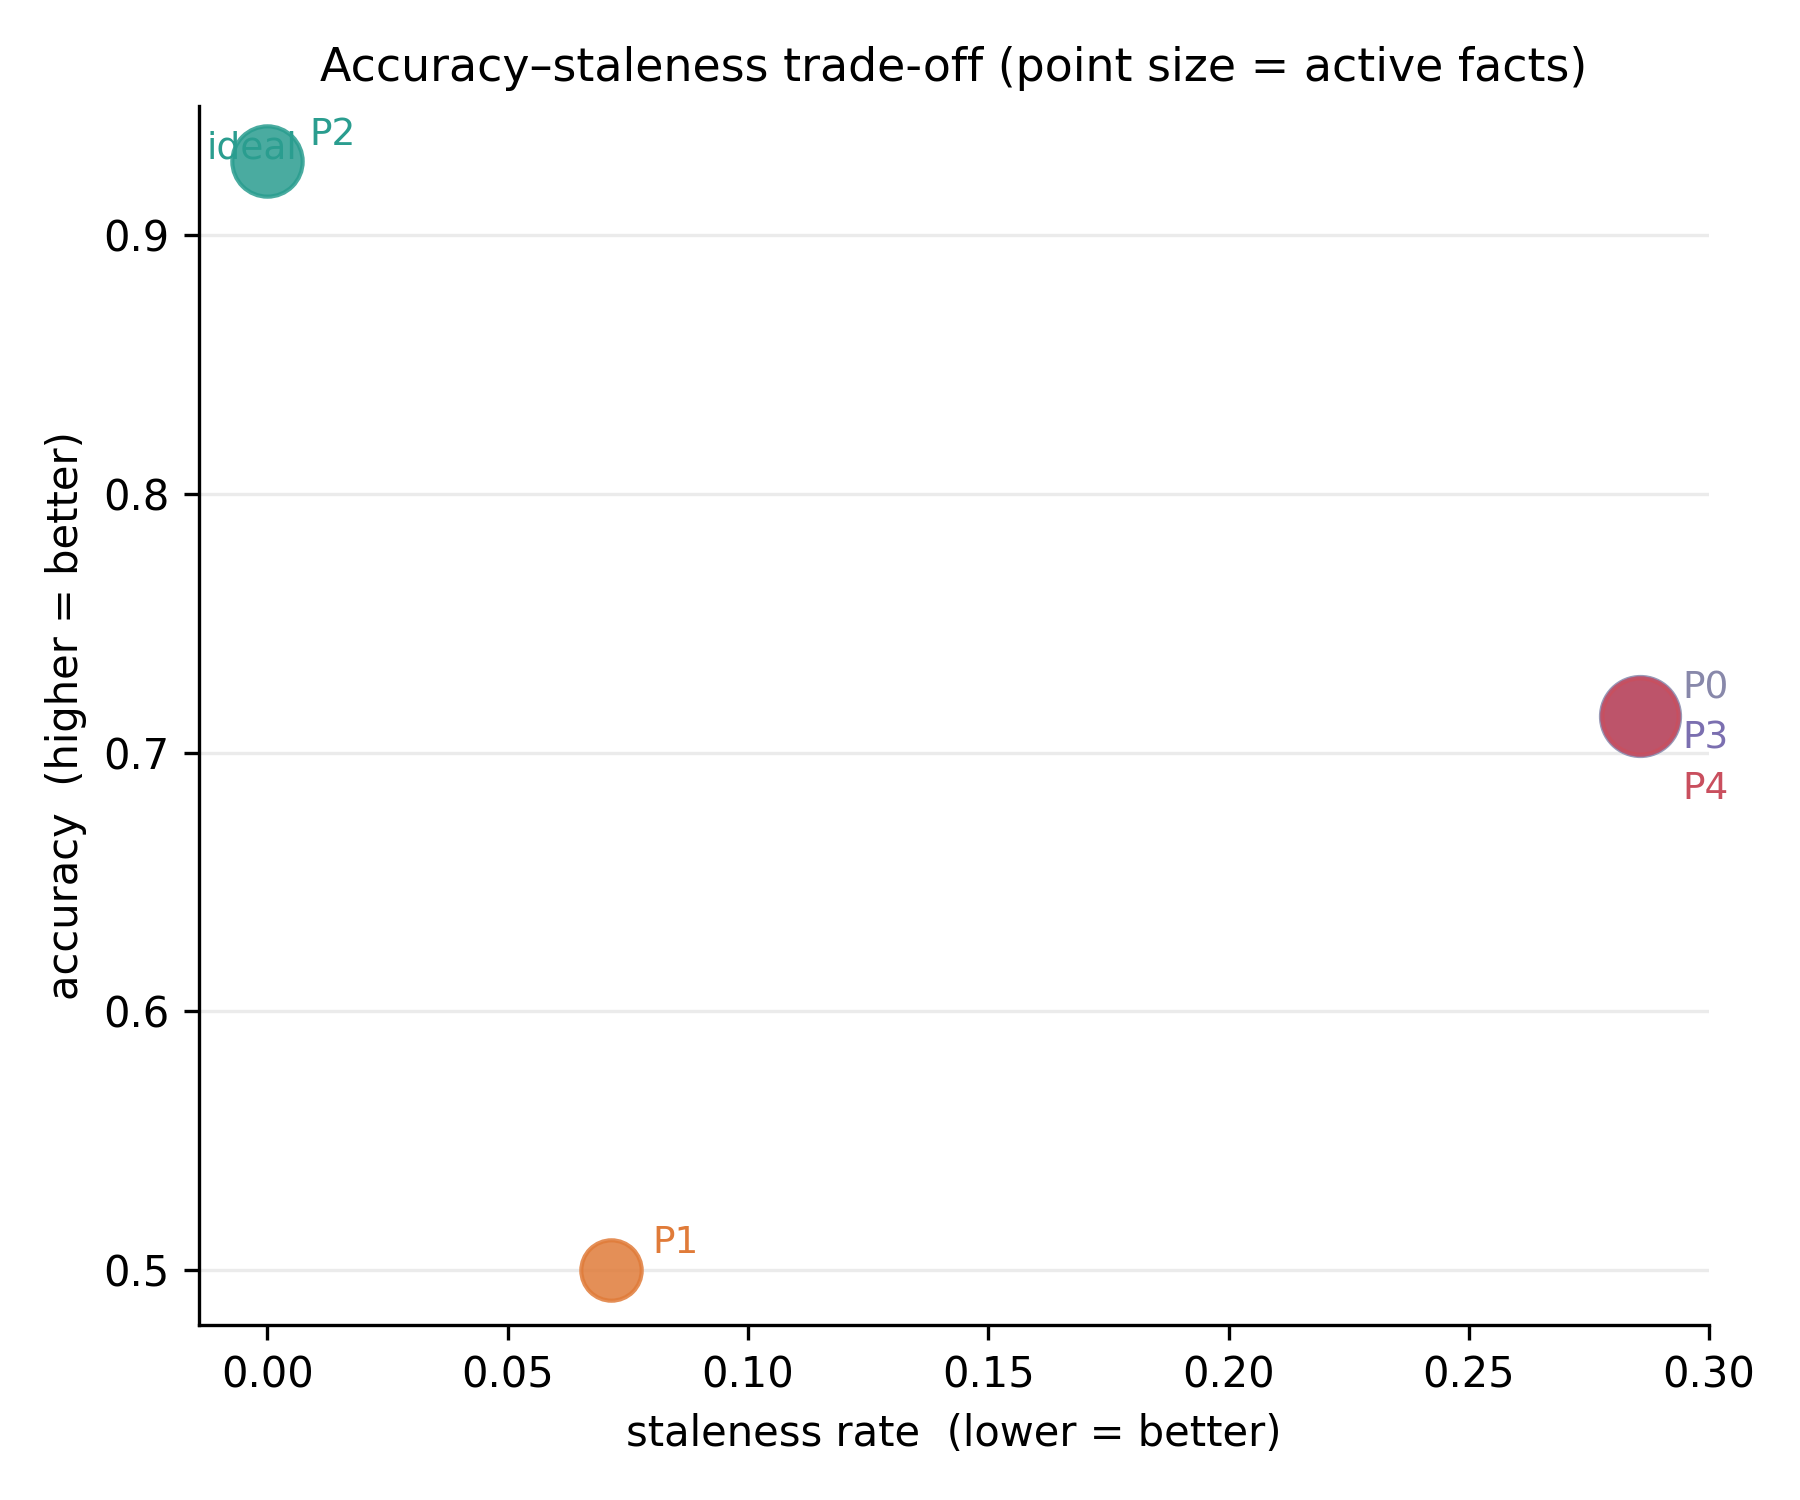
\includegraphics[width=0.95\columnwidth]{figures/tradeoff_scatter.png}
\caption{Accuracy against staleness for the controlled study. The ideal region is the top left. Point size is proportional to active memory size.}
\label{fig:tradeoff}
\end{figure}

\paragraph{The ranking survives multi-agent usage.} Table~\ref{tab:swarm} reports the same policies under the three topologies. The ordering P2 $>$ P0 $\approx$ P3 $\approx$ P4 $>$ P1 is unchanged in all three. Two observations stand out. First, in the shared topology every invalidation was cross-writer: the update arrived through a different agent than the original fact, and P2's accuracy did not move. Contradiction detection lives in the graph rather than in any agent, so it is writer-agnostic by construction. Second, TTL decay collapses to 0.143 accuracy under the interleaved timeline, because the global session stream spans the full 58 days and a fixed TTL prunes nearly everything old, including facts that are still true. The failure mode of time-based forgetting grows with exactly the long horizons that motivate forgetting in the first place.

\begin{table}[t]
\centering
\small
\begin{tabular}{@{}lccc@{}}
\toprule
Policy & Shared & Independent & Orchestr. \\
\midrule
P0 & 0.714 & 0.667 $\pm$ 0.041 & 0.714 \\
P1 & 0.143 & 0.143 $\pm$ 0.000 & 0.143 \\
P2 & \textbf{0.929} & \textbf{0.881 $\pm$ 0.041} & \textbf{0.929} \\
P3 & 0.714 & 0.667 $\pm$ 0.041 & 0.714 \\
P4 & 0.714 & 0.667 $\pm$ 0.041 & 0.714 \\
\bottomrule
\end{tabular}
\caption{Accuracy under three multi-agent topologies (controlled study, three agents). Independent reports mean and standard deviation over agents with 80\% observation. Staleness is 0.286 for P0, P3, P4 and 0.000 for P1, P2 in all topologies.}
\label{tab:swarm}
\end{table}

\paragraph{Partial observation degrades gracefully.} In the independent topology, an agent that missed the session containing an update cannot invalidate the old fact, so P2's mean accuracy drops from 0.929 to 0.881 with small variance. The degradation is proportional to what was missed and does not affect agents that observed the update.

\begin{figure}[t]
\centering
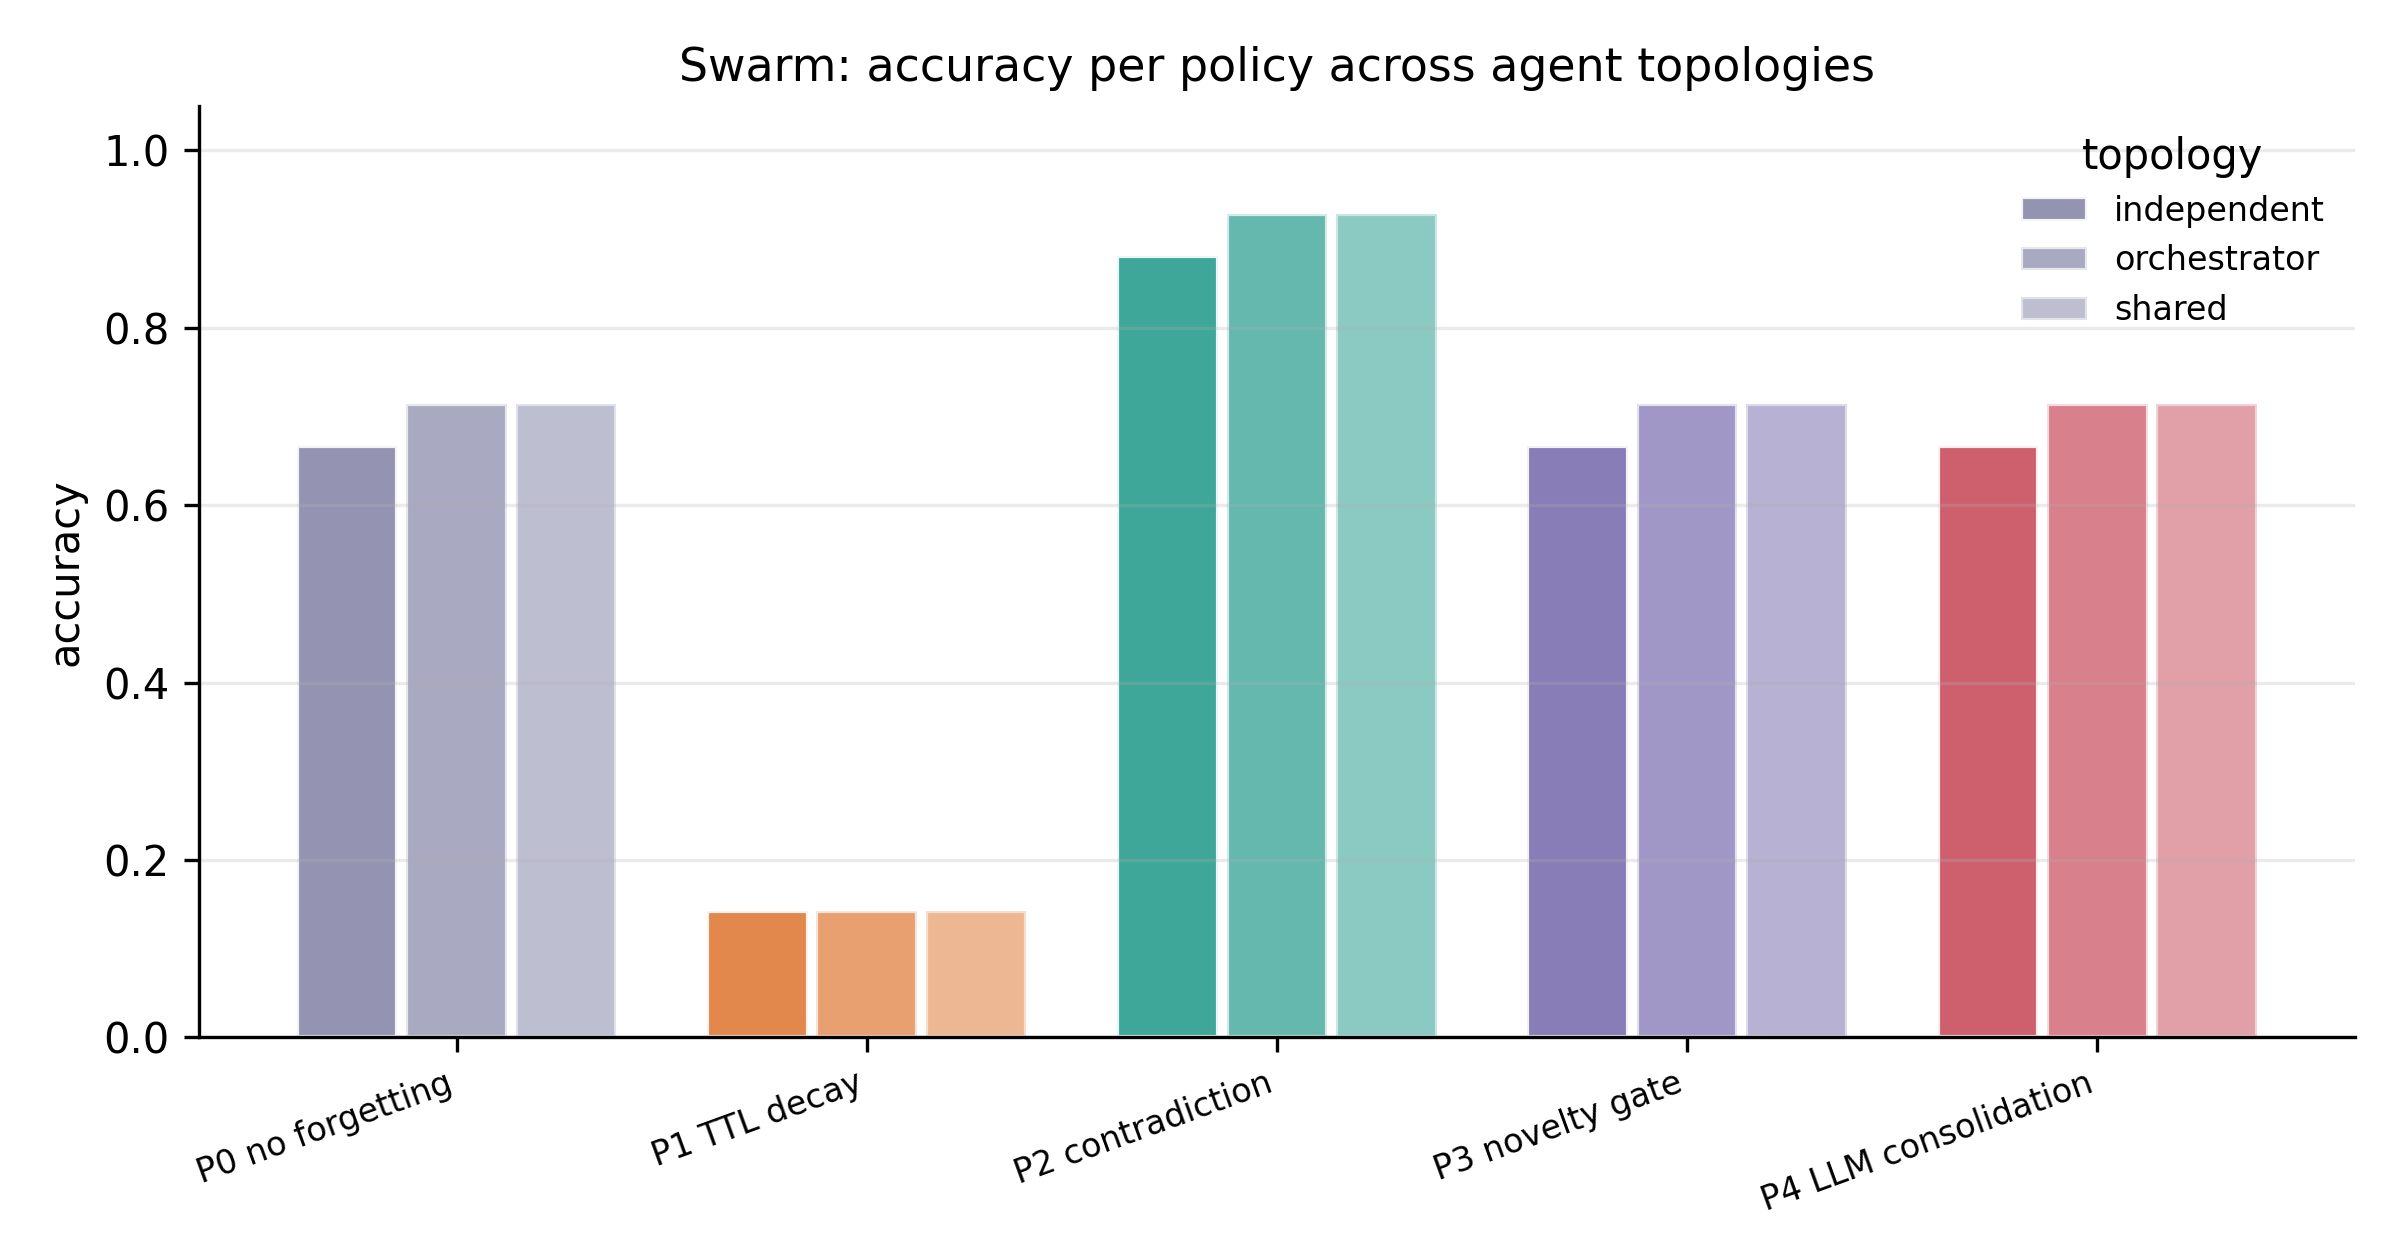
\includegraphics[width=0.95\columnwidth]{figures/swarm_topology.png}
\caption{Accuracy per policy across the three agent topologies in the controlled study. The policy ranking is invariant to topology.}
\label{fig:swarm}
\end{figure}

\paragraph{Real-model experiments.} We are running the full matrix of 6 policies, 5 answer-model families, and both public benchmarks, together with a five-agent model-diverse shared-memory configuration. All cells are resumable and cached.
% ------------------------------------------------------------------
% TODO (before submission): insert the LoCoMo main table here
% (results/locomo/summary_table.json), the LongMemEval knowledge-update
% breakdown (results/longmemeval/), the model-comparison figure
% (results/locomo/figures/model_comparison.png), and the five-agent
% swarm table (results/swarm_real/summary_table.json). Update the
% abstract and this paragraph to state the real-model findings.
% ------------------------------------------------------------------

\section{Discussion}

The controlled results support a simple reading: forgetting is not one mechanism but three intervention points, and the intervention that improved correctness is the one that consumes information the substrate already has. P2 contains no learned component and makes no model calls. Its advantage comes entirely from the representation, the validity interval that a contradiction closes. The ablation sharpens this: P5 uses the same graph and a reasonable structural heuristic, ignores time, and lands below the append-only baseline. If these findings hold on the real-model matrix, the practical advice to system builders is concrete. Implement contradiction-driven invalidation at retrieval time before investing in consolidation by a language model, which costs tokens and, consistent with \citet{zhang2026faulty}, carries real risk.

The multi-agent invariance result also has a practical corollary. Because supersession is recorded in the shared graph, memory hygiene does not require agents to coordinate or even to know about each other. This is relevant to the failure modes that \citet{ren2026gatemem} report for shared memories, where stale values propagate between principals.

\section{Limitations}

The controlled study uses a small synthetic benchmark and a deterministic answerer. It validates the mechanism and the harness, not generality; the real-model matrix on LoCoMo and LongMemEval is the test of generality, and this paper should be evaluated together with those results. Contradiction detection relies on a fixed list of functional predicates and string-based entity matching, so a real extractor that misses a predicate removes P2's advantage on that fact; our extraction pipeline includes a deterministic normalization pass to reduce this dependence, but it does not eliminate it. The judge in real runs is a language model with known biases, which we mitigate by using a different vendor family and reporting token F1. Finally, our staleness metric requires annotated superseded answers, which exist in our synthetic data and in LongMemEval's knowledge-update category but not in most benchmarks.

\section{Conclusion}

We asked when agents should forget, and built a framework where the question has a controlled answer. On a bitemporal knowledge graph, forgetting driven by recorded contradictions removed staleness completely, preserved old knowledge, cost nothing at inference time, and kept its advantage when five heterogeneous agents shared one memory. Time-based decay, novelty gating, consolidation by a language model, and time-blind structural consolidation each failed in a different and now measurable way. The broader lesson we draw is that memory hygiene is primarily a representation problem. When the store records validity in time, the right forgetting policy is close to trivial; when it does not, no scoring heuristic we tested recovers the difference.

\section{Acknowledgments}

This work was carried out as part of a Masters thesis in Applied AI. We thank the maintainers of the open inference providers whose free tiers made the experiments possible.

\bibliography{drift_paper}

\end{document}
